\section{Verification}

\subsection{Core Components Unit Tests}

Here I give some small unit tests for some of the smaller core components of the program, things like the Logger and some of the physics objects like four-vectors.

\subsubsection{Logger}

The unit tests here are minimal; all we need to test is that the four types of errors print as they should and handle the printing of various data types.

\begin{listing}
  \begin{minted}{cpp}
#include <ColSim/ColSim.hpp>
using namespace ColSim;

#include <string>
using namespace std;

int main() {

  LOGGER.logMessage("This is a message.");
  LOGGER.logWarning("This is a warning.");
  LOGGER.logError("This is an error that will NOT abort the program.");

  string str = "this is a string!";
  LOGGER.logMessage("String: %s", str.c_str());

  int x = 42;
  LOGGER.logMessage("Integer: %d", x);

  double y = 5.679122;
  LOGGER.logMessage("Double: %.5lf", y);

  LOGGER.logAbort("This is an error that will abort the program.");

  return 0;
}
  \end{minted}
  \caption{Test program to testing logging functionality.}
  \label{listing:logger-tests}
\end{listing}

\begin{figure}[ht]
  \centering
  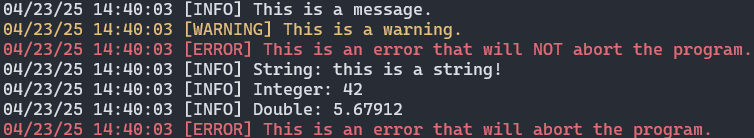
\includegraphics[width=0.7\linewidth]{./res/gfx/logger-tests.png}
  \caption{Output from the code given in Listing~\ref{listing:logger-tests}}
  \label{fig:logger-tests}
\end{figure}

The code used to test the logger is given in Listing~\ref{listing:logger-tests} and the output is given in Figure~\ref{fig:logger-tests}. Evidently, the logger is performing as expected.

\subsubsection{Settings}

The Settings functionality will also be similar to test. All input variables have a default value, so the behavior for them all is that if they are neglected from the config file, no warnings/errors occur, rather the default value is set for that parameter. This can be illustrated by a simple test case as shown in Table~\ref{tbl:settings-test1}. A few variables, such as the aforementioned cutoff scales, have hard limits and cannot be configured below $1.0$, otherwise the program will crash. It also will emit warnings if the the cutoff is set too high, as this often reduces the accuracy of the calculation. These cases are given in Table~\ref{tbl:settings-test2}.

\begin{table}[ht]
  \centering
  \begin{tabular}{|c|c|}
    \hline
    \textbf{Action} & Keeping/removing $E_{\mathrm{ECM}}$ from the config file. \\ \hline
    \textbf{Expected Output} & If omitted, keeps $\qty{14}{\giga\electronvolt}$, otherwise uses specified value. \\ \hline
    \textbf{Actual Output (Omitted)} & 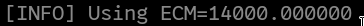
\includegraphics[width=0.5\textwidth]{./res/gfx/settings-test1a.png} \\ \hline
    \textbf{Actual Output (Specifying $12.5$)} & 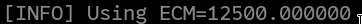
\includegraphics[width=0.5\textwidth]{./res/gfx/settings-test1b.png} \\ \hline
  \end{tabular}
  \caption{Test case for omitting $E_{\mathrm{ECM}}$ from the configuration file.}
  \label{tbl:settings-test1}
\end{table}

\begin{table}[ht]
  \centering
  \begin{tabular}{|c|c|}
    \hline
    \textbf{Action} & Specifying a value $<1.0$ and $>50.0$ for the parton evolution cutoff scale. \\ \hline
    \textbf{Expected Output} & For $<1.0$, aborts, for $>50.0$, gives warning. \\ \hline
    \textbf{Actual Output ($<1.0$)} & 
\includegraphics[width=0.75\textwidth]{./res/gfx/settings-test2a.png} \\ \hline
    \textbf{Actual Output ($>50.0$)} & 
\includegraphics[width=0.75\textwidth]{./res/gfx/settings-test2b.png} \\ \hline
  \end{tabular}
  \caption{Test case for violating ranges for parton evolution cutoff energy.}
  \label{tbl:settings-test2}
\end{table}

Evidently, the settings interface seems to be performing as expected, and aborts upon specifying parameters that are completely incompatible with the model (and underlying theory), and warns if parameters are specified that are in principle allowed, but may lead to less accurate results.


\subsubsection{Four-Vectors}

The testing for four-vectors is relatively simple: the only non-trivial functionality of four-vectors is to ensure that the calculation of the transverse momentum components, i.e. $p_T^2 = p_x^2 + p_y^2$, is performed correctly, the calculation of the norm $p_\mu p^\mu \equiv p_0^2 - p_x^2 - p_y^2 - p_z^2$ is performed correctly, and boosts along the $z$-axis (the beam axis). A boost is defined by a parameter $\beta$ which is the fraction of the speed of light to boost the particle. Defining

\begin{equation}
  \gamma = \sqrt{\frac{1}{1-\beta^2}},
\end{equation}

the boost is given by

\begin{equation}
  p^\mu \rightarrow p^{\mu\prime} = \begin{pmatrix}\gamma (p_0 - \beta p_z) & p_x & p_y & \gamma(p_z - \beta p_0)\end{pmatrix}.
\end{equation}

We choose some random values for the components:

\begin{equation}
  p^\mu = \begin{pmatrix}89.0 & 5.9 & 3.4 & 9.8\end{pmatrix}.
\end{equation}

\begin{table}[ht]
  \centering
  \begin{tabular}{|c|c|c|}
    \hline
    Quantity & Expected & Actual \\ \hline
    $p_T^2$ & $7778.59$ & $7778.59$ \\ \hline
    $p_\mu p^\mu$ & $46.37$ & $46.37$ \\ \hline
    Boost of $\beta = 0.5$ & $p^\mu = (42.05,\ 5.9,\ 3.4,\ 412.85)$ & $p^\mu = (42.05,\ 5.9,\ 3.4,\ 412.85)$ \\ \hline
  \end{tabular}
  \caption{Calculated and expected values for calculated quantities involving four-vectors.}
  \label{tbl:four-vector-tests}
\end{table}

Table~\ref{tbl:four-vector-tests} contains the result from this test. Clearly, we are computing the correct values for four-vectors.

\subsubsection{Gnuplot}

The interface for plotting things with Gnuplot is less of a concrete test but rather that it can handle plotting some generic function. Due to the histogram format of the plotting that is done for the rest of the program, I do a mini Monte-Carlo to essentially plot $sin^2(x)$ between $0-\pi$. The listing is a little long, so it given as Listing~\ref{listing:gnuplot-testing} in Appendix~\ref{sec:gnuplot-listing}.

\begin{figure}[ht]
  \centering
  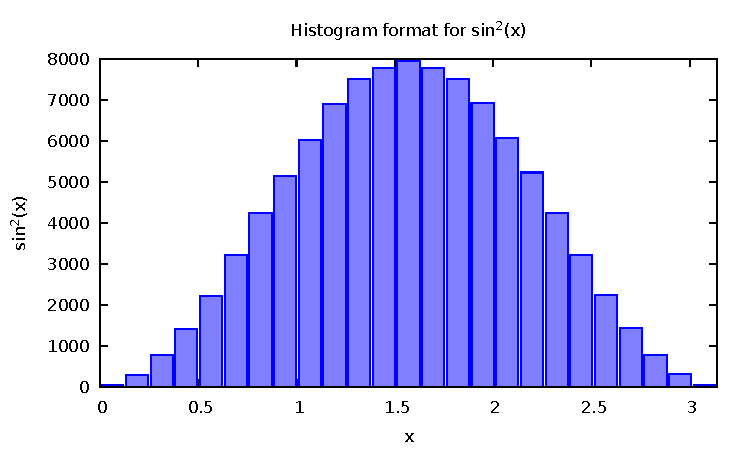
\includegraphics[width=0.75\linewidth]{./res/gfx/sin2_x.pdf}
  \caption{Histogram form for the plot of $sin^2(x)$.}
  \label{fig:sin2x}
\end{figure}

The plot for the resulting distribution is given in Figure~\ref{fig:sin2x}. The code for the Gnuplot interface therefore works as expected, and is relatively easy to use.





\subsection{Monte Carlo Unit Test}

A simple unit test of the Monte Carlo algorithm is conducted by running the algorithm using a few simple functions that can be calculated analytically. Since there is no reason for the algorithm to work for simple functions but fail for complex functions, I have selected a few easy functions that are easy to integrate analytically (or otherwise have exact known results):

\renewcommand{\arraystretch}{1.5}
\begin{table}[ht]
  \centering
  \begin{tabular}{|c|c|c|c|c|}
    \hline
    Integral & Monte Carlo Result & Error & Exact Value & Relative Error \\ \hline
    $\int_0^1\dd x \; 2x$ & $1.0002$ & $\pm \num{5.774d-4}$ & $1.0$ & $\qty{.022}{\percent}$ \\ \hline
    $4\int_0^1 \frac{\dd x}{1+x^2}$ & $3.14164$ & $\pm \num{6.435d-4}$ & $\pi$ & $\qty{1.42d-3}{\percent}$ \\ \hline
    $\int_{-\infty}^\infty \dd x\dd y\dd z e^{-(x^2+y^2+z^2)}$ & $5.8080$ & $\pm 0.122$ & $\pi^{3/2}$ & $\qty{6.59}{\percent}$ \\ \hline
  \end{tabular}
  \caption{Test functions to ensure Monte Carlo convergence.}
  \label{tbl:monte-carlo-tests}
\end{table}
\renewcommand{\arraystretch}{1.0}

The results are shown in Table~\ref{tbl:monte-carlo-tests}. The first two functions are simple analytic functions and they yield less than a tenth of a percent relative error between the exact values and those determined from the Monte Carlo algorithm. The third function is a Gaussian, and due to the nature of the limits being $\pm\infty$, it is much harder to accurately assess the integral with smaller numbers of iterations. There are techniques to mitigate this, but the integrals that I compute do not have this feature, so I do not think it is necessary to fix anything. It is interesting to see, though, where the Monte Carlo algorithm breaks down. Despite this, like I just mentioned, the integrals I compute are finite, meaning the algorithm's convergence is very good and it works as intended.

These are the main sub-components within the project. There are a few more super minor utility functions and other things, but these are insignificant enough to not necessarily require unit testing.

\subsection{Physics Components}

The issue with trying to unit test the physics components is that, at the end of the day, the main part of the hard scattering process revolves directly around the Monte Carlo algorithm. We have shown that that works very well. The remaining physics component is, in the context of this milestone, implementing the equations that are calculated with the Monte Carlo algorithm. Therefore, there really is no remaining unit testing to be done with respect to the hard scattering.

With respect to the parton showering, the Sudakov form factor is the main driving component. This, however, is less of a general algorithm like Monte Carlo, but instead is implemented directly for this case. Therefore, the only testing that can be done is on the entire unit as a whole, which has already been done in the previous main section.

Therefore, this concludes the unit testing for the main sections of the progam. It is evident that the individual components work well on their own and can withstand different inputs being presented.




\subsection{Regression Testing}

I am unsure what to write for this section. The behavior of the above individual components have worked from the get-go, with only interface changes; i.e. the Monte Carlo algorithm has always worked, the Gnuplot interface has always plotted the functions, with, again, only minor API changes. Therefore, there is nothing to really document for this testing case, but rather, the documentation changes will be reflected in the main program documentation.



\subsection{Edge Case Testing}

This has already been conducted in the previous section and the previous milestone, specifically in the case of the Settings testing and varying of the input parameters. Specific limits have already been tested and described thoroughly in the previous section, which are the edge cases this section refers to. Therefore, refer to that section and Milestone 6 for the edge case behavior.



\subsection{Integration Testing}

Integration testing is challenging, because any integrations of the above individual components are already present in the main output that I have already extensively discussed. Therefore, considering that the model performance overall considering both the numerical results and also the simple fact that the output is readable, nothing crashes, etc., I think the integration testing is more or less satisfied.




\subsection{Code Review}

A big (and apparently controversial) opinion of mine is that code readability is entirely subjective. If one is working on a large project with a number of collaborators, it's must consider the practices of the collaborators, but this project is one I am programming myself. Therefore, readability is entirely my own preference, and has been written from the get-go with my own best practices I have been refining throughout my career.

In terms of actual coding practices as they relate to C++ programming, I have enabled all possible warnings and extra warnings during the compilation, i.e. via the \texttt{-Wall -Wextra} flags to the \texttt{g++} compiler. These have ensured that improper (not \textit{unreadable}) code is avoided as much as possible. The current state of the code compiles in its entirety with zero warning (and of course zero errors).


\subsection{Version Control}

The code can be found on GitHub \href{https://github.com/champso1/ColSim}{here}. The version controlling has been very poor recently, as the majority of the work has been spent running tests and whatnot. Further, my version controlling via Git has not been the best in general, which is something that I have to improve on. 









%%% Local Variables:
%%% mode: LaTeX
%%% TeX-master: "../../Milestone7"
%%% End:
